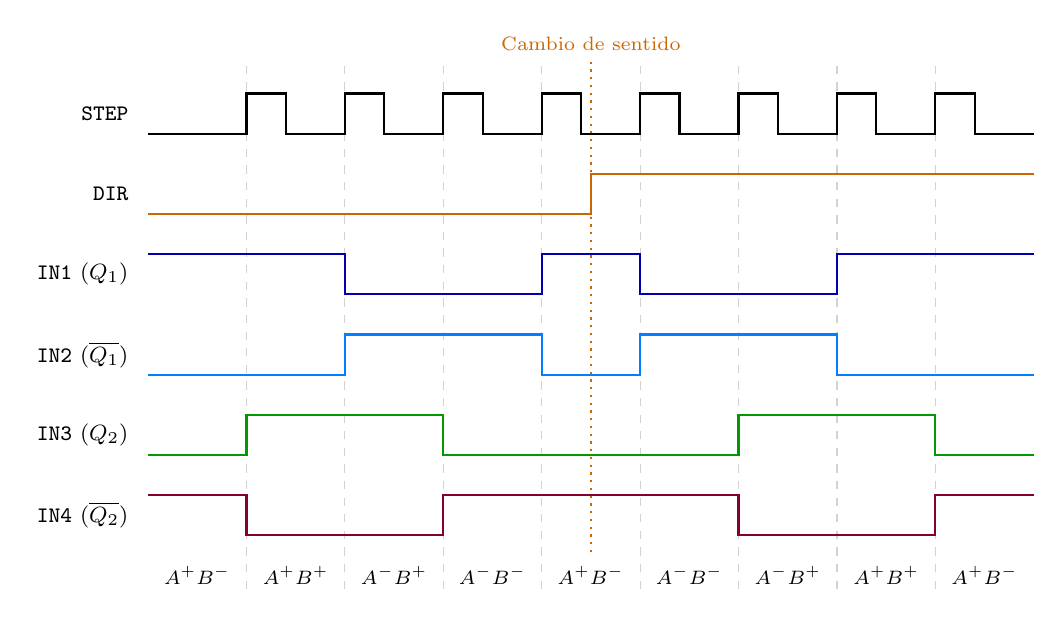
\begin{tikzpicture}[x=1.25cm, y=0.85cm, font=\footnotesize]
  % Grilla vertical de referencia en cada flanco ascendente de STEP
  \foreach \x in {1,2,3,4,5,6,7,8} {
    \draw[gray!35, dashed] (\x, -0.3) -- (\x, 7.6);
  }
  % Linea de cambio de DIR (termina sobre las etiquetas de estado)
  \draw[orange!80!black, dotted, thick] (4.5, 0.25) -- (4.5, 7.6);

  % Etiquetas de canales a la izquierda
  \node[left] at (-0.1, 6.8) {\texttt{STEP}};
  \node[left] at (-0.1, 5.6) {\texttt{DIR}};
  \node[left] at (-0.1, 4.4) {\texttt{IN1} ($Q_1$)};
  \node[left] at (-0.1, 3.2) {\texttt{IN2} ($\overline{Q_1}$)};
  \node[left] at (-0.1, 2.0) {\texttt{IN3} ($Q_2$)};
  \node[left] at (-0.1, 0.8) {\texttt{IN4} ($\overline{Q_2}$)};

  % STEP (pulsos en t = 1..8)
  \draw[thick, black]
    (0,6.5) -- (1,6.5) -- (1,7.1) -- (1.4,7.1) -- (1.4,6.5) --
    (2,6.5) -- (2,7.1) -- (2.4,7.1) -- (2.4,6.5) --
    (3,6.5) -- (3,7.1) -- (3.4,7.1) -- (3.4,6.5) --
    (4,6.5) -- (4,7.1) -- (4.4,7.1) -- (4.4,6.5) --
    (5,6.5) -- (5,7.1) -- (5.4,7.1) -- (5.4,6.5) --
    (6,6.5) -- (6,7.1) -- (6.4,7.1) -- (6.4,6.5) --
    (7,6.5) -- (7,7.1) -- (7.4,7.1) -- (7.4,6.5) --
    (8,6.5) -- (8,7.1) -- (8.4,7.1) -- (8.4,6.5) -- (9,6.5);

  % DIR (0 para t < 4.5, 1 para t >= 4.5)
  \draw[thick, orange!80!black]
    (0,5.3) -- (4.5,5.3) -- (4.5,5.9) -- (9,5.9);

  % IN1 = Q1: [0,2]=1, [2,4]=0, [4,5]=1, [5,7]=0, [7,9]=1
  \draw[thick, blue!70!black]
    (0,4.7) -- (2,4.7) -- (2,4.1) -- (4,4.1) -- (4,4.7) --
    (5,4.7) -- (5,4.1) -- (7,4.1) -- (7,4.7) -- (9,4.7);

  % IN2 = /Q1: [0,2]=0, [2,4]=1, [4,5]=0, [5,7]=1, [7,9]=0
  \draw[thick, blue!50!cyan]
    (0,2.9) -- (2,2.9) -- (2,3.5) -- (4,3.5) -- (4,2.9) --
    (5,2.9) -- (5,3.5) -- (7,3.5) -- (7,2.9) -- (9,2.9);

  % IN3 = Q2: [0,1]=0, [1,3]=1, [3,6]=0, [6,8]=1, [8,9]=0
  \draw[thick, green!60!black]
    (0,1.7) -- (1,1.7) -- (1,2.3) -- (3,2.3) -- (3,1.7) --
    (6,1.7) -- (6,2.3) -- (8,2.3) -- (8,1.7) -- (9,1.7);

  % IN4 = /Q2: [0,1]=1, [1,3]=0, [3,6]=1, [6,8]=0, [8,9]=1
  \draw[thick, purple!70!black]
    (0,1.1) -- (1,1.1) -- (1,0.5) -- (3,0.5) -- (3,1.1) --
    (6,1.1) -- (6,0.5) -- (8,0.5) -- (8,1.1) -- (9,1.1);

  % Estados resultantes por intervalo
  \node[font=\scriptsize] at (0.5, -0.1) {$A^+ B^-$};
  \node[font=\scriptsize] at (1.5, -0.1) {$A^+ B^+$};
  \node[font=\scriptsize] at (2.5, -0.1) {$A^- B^+$};
  \node[font=\scriptsize] at (3.5, -0.1) {$A^- B^-$};
  \node[font=\scriptsize] at (4.5, -0.1) {$A^+ B^-$};
  \node[font=\scriptsize] at (5.5, -0.1) {$A^- B^-$};
  \node[font=\scriptsize] at (6.5, -0.1) {$A^- B^+$};
  \node[font=\scriptsize] at (7.5, -0.1) {$A^+ B^+$};
  \node[font=\scriptsize] at (8.5, -0.1) {$A^+ B^-$};

  \node[above, font=\scriptsize, orange!80!black] at (4.5, 7.6) {Cambio de sentido};
\end{tikzpicture}
